\documentclass[11pt]{article}
%\usepackage{ngerman}
\usepackage[english]{babel}
\usepackage{amsmath,amssymb,amstext}
\usepackage{graphicx}
\usepackage{parskip}
\usepackage{float}
\usepackage{tabularx}
\usepackage{amsmath}
\usepackage{esint}
%\usepackage{subtextbf}
\usepackage{pdfpages}
\usepackage{url}
%\usepackage{cite}
\usepackage{array}
\usepackage{multirow}
\usepackage{hyperref}
\usepackage{biblatex}


 
\bibliography{Documentation/references/references}
\bibliographystyle{plain}
\setlength{\textwidth}{15 true cm}
\setlength{\textheight}{22 true cm}
\oddsidemargin  0.5 cm
\evensidemargin 0.5 cm
\topmargin      0 cm

\renewcommand{\textfraction}{.2}
\renewcommand{\floatpagefraction}{.8}

\begin{document}
%\frontmatter
\pagenumbering{roman}

% Include titlepage
\begin{titlepage}	
	{\sffamily		
		\begin{center}			
			
\includegraphics[width=30mm]{images/TU_Graz_Logo.png}
			
			\vfill\vfill\vfill
			\vfill\vfill\vfill
			
			{Simon Prato}
			% Author with existing titles
			
			\vfill\vfill\vfill
			
			{\LARGE\bfseries{Title}}
			% Title of the thesis			
			
			\vfill\vfill\vfill
			\vfill\vfill\vfill			
			
			{\bfseries\large{Master Thesis}}
			
			{Studies: {Electrical Engineering}}
						
			\vfill\vfill\vfill			
			
			submitted to
			
			\vfill
			
			{\bfseries\large{Technical University of Graz}}			
			
			\vfill\vfill\vfill			
			
			Supervisor
			
			{Dr. Thomas Bauernfeind}
			
			\vfill
			
			\vfill
			
			
\includegraphics[width=30mm]{Documentation/images/igte_logo.png}
			
			%% OPTIONAL: second supervisor/name of the faculty, etc.
					
			\vfill\vfill\vfill
					
			{Graz}, {August}~{2024}
			
		\end{center}
	}%% end sffamily
\end{titlepage}

\newpage

% Kurzfassung
\iftrue
\cleardoublepage
\setcounter{page}{2}
\vspace*{2.2 cm}
{\Large
\noindent
{\bf Abstract}} \\
\vspace*{0.3 cm}

\noindent

% Abstract
\cleardoublepage
\fi

\selectlanguage{english}
% Inhaltsverzeichnis
	\tableofcontents  

% Tabellenverzeichnis
% optional
\newpage
	\listoffigures 

% Abbildungsverzeichnis
% optinal
\newpage
	\listoftables
	
\cleardoublepage

%\mainmatter
\pagestyle{headings}
\pagenumbering{arabic}

\section{Introduction}

\section{Theoretical Basics}
\subsection{Dipoles}
\subsubsection{Electric Dipoles}

Modeling the electromagnetic radiation of antennas proves to be a challenging task. Using magnetic and electric dipoles is a way to do this, which is especially well applicable for electrically small antennas, which are used in this document. Electrically small antennas have dimensions which are less than one tenth of the wavelength ($<<\frac{\lambda}{10}$)\cite{Balanis_1997}. By calculating the respective dipole moments, the coupling of the antennas to the TEM cells is numerically estimated. Therefore, this section aims to provide a short introduction to the theory behind this concept.

An electric dipole is often described as two tiny charged metal spheres, which are connected with a linear and thin wire\cite{Griffiths_2024} or simply as an T-antenna containing charged capacitor-plates at the end of the wire \cite{Balanis_1997}. The distance $d$ between those charges is very short compared to the wavelength ($d << \lambda$), therefore the dipole can be approximated as ideal\cite{Griffiths_2024}. The electric dipole moment $\mathbf{p}$ is defined by \autoref{eqn:elec_dipole_mom}\cite{Balanis_1997}\cite{Jackson}. %% Erklärung hier. Besser die Bücher zu referenzieren, als selbst etwas zu erfinden.

\begin{equation}
    \mathbf{p} = \int\mathbf{x'} \rho (\mathbf{x'})\mathrm{d}^3x'
    \label{eqn:elec_dipole_mom}
\end{equation}

\autoref{fig:electric_dipole} demonstrates a simple example of a center-fed dipole with a narrow gap as a feedpoint, for which the electric dipole can be used to calculate its radiation\cite{Griffiths_2024}\cite{Jackson}. A current $I_0$ is injected at the feedpoint, which linearly drops to zero along the antenna arms, as described by \autoref{eqn:current_dipole}\cite{Jackson}.

\begin{equation}
    I(z)= I_0\left( 1-\frac{2|z|}{d} \right)
    \label{eqn:current_dipole}
\end{equation}

%Hier das Ergebnis der Integration anschreiben. Die integration selbst auch anschreiben- 

\begin{figure}[h]
    \centering
    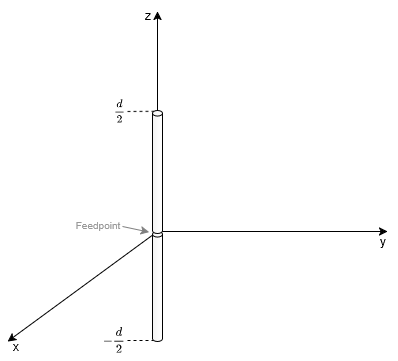
\includegraphics[width=0.5\linewidth]{Documentation//images/electric_dipole_drawing.png}
    \caption{Electric dipole}
    \label{fig:electric_dipole}
\end{figure}

The charge per unit length $\rho'$, approximated due to the thin wire, is then derived by the continuity equation in frequency domain by \autoref{eqn:charge_distribution_dipole}. It is constantly distributed along each antenna arm\cite{Griffiths_2024}\cite{Jackson}.

\begin{equation}
    \rho' = \pm\frac{\mathrm{d}}{\mathrm{d}z}\frac{\mathrm{i}I(z)}{\omega} = \pm\frac{2\mathrm{i}I_0}{\omega d}
    \label{eqn:charge_distribution_dipole}
\end{equation}

Using \autoref{eqn:elec_dipole_mom} leads to the resulting electric dipole moment in \autoref{eqn:dipole_mom_example} of this structure. It is parallel to the antenna's arms and points in z-direction\cite{Griffiths_2024}\cite{Jackson}. 

\begin{equation}
    \mathbf{p}=\int_{-\frac{d}{2}}^{\frac{d}{2}}z\rho'(z)\mathrm{d}z\cdot\mathbf{e}_z = \frac{\mathrm{i}I_0d}{2\omega}
    \label{eqn:dipole_mom_example}
\end{equation}

Next, the vector potential $\mathbf{A}$ is determined, to further derive any radiation. It is defined in \autoref{eqn:vector_pot}\cite{Balanis_1997}\cite{Jackson}. % Eventuell extra in einem anderen Kapitel diese Bascis anschreiben. 

\begin{equation}
    \mathbf{A}(\mathbf{x})=\frac{\mu}{4\pi}\frac{\mathrm{e}^{\mathrm{i}kr}}{r}\int \mathbf{J}(\mathbf{x'})\mathrm{d}^3x'
    \label{eqn:vector_pot}
\end{equation}

The vector potential $\mathbf{A}$ of an electric dipole is calculated with \autoref{eqn:vector_pot_elec_dipole}\cite{Jackson}.

\begin{equation}
    \mathbf{A} (\mathbf{x})=-\frac{\mathrm{i\mu_0\omega}}{4\pi}\mathbf{p}\frac{\mathrm{e}^{\mathrm{i}kr}}{r}
    \label{eqn:vector_pot_elec_dipole}
\end{equation}
Should the calculation of fields even be included? I don't need them for research. But the Field equations are important for explaining the frequency behavior of the electric dipole moment. This can be done by the radiation resistance in \autoref{eqn:elec_rad_res}. In our example, the radiation power depends on the frequency squared ($\mathbf{p}$\textasciitilde
$\frac{1}{f}$ and $k$ \textasciitilde $f$, leading to $P_{rad}$ \textasciitilde $f^2$ overall)\cite{Jackson}. Therefore, it is to be expected that the small electric dipole leads to increased coupling with the TEM cell by frequency squared.

\begin{equation}
    P_{rad} = \frac{\mathrm{c}^2\mathrm{Z_0}\mathrm{k}^4}{12\pi}|\mathbf{p}|^2
    \label{eqn:elec_rad_res}
\end{equation}

The electric dipole described in this section approximate the real behavior of electrically short antennas. However, special care must be taken of the excitation method and shape, as it influences the results heavily\cite{Jackson}. Additionally, any antenna investigated through this method must remain as small as possible compared to the wavelength $\lambda$, to reduce any analytical approximation errors. 

The electric field increases quadratically with frequency.... Hence electric dipole moment increases over frequency... Write about that -> Griffiths

% Next, the electric and magnetic fields, how the dipole moment is calculated with this and how ansys HFSS uses this. Look also in the other two ressources, the other two books. Ansys HFSS handles them as physical dipole antennas? Maybe add radiation pattern. Additionally, describe how the electric field odminates in electric dipoles. In Dominik's paper, the magnetic coupling dominates, because of the magnetic dipole.

The behavior of the electric dipole may be divided into three categories\cite{Griffiths_2024}\cite{Jackson}:
\begin{enumerate}
    \item The near zone, 
\end{enumerate}

\subsubsection{Magnetic Dipoles}

The magnetic dipole is represented by a current loop with a radius $b$. Its axis is perpendicular to the plane of the loop. Its field radiated are the same as in the electric dipole, but with the electric and magnetic fields reversed\cite{Balanis_1997}. The magnetic dipole moment is given by \autoref{}

\begin{equation}
    \mathbf{m}=\frac{1}{2}\int (\mathbf{x} \times \mathbf{J})\mathrm{d}^3x
\end{equation}


\subsubsection{Combination of Dipoles}
% Read Bauernfeind's: Crossed Dipole Antennas

When placing the magnetic dipole in the center of the upper or lower chamber of the TEM cell, and pointing in y-direction, it will generate a TEM-wave. Same goes for the electric dipole, pointing in z-direction. When combining two of these dipole moments, any excitation with the first order TEM mode is possible. This is the main idea for modeling antennas. The relation of the magnetic and electric fields is assumed to be roughly equal to the free space wave impedance. Also, magnetic dipoles create a difference in output voltage of the two ports, while electric dipoles create a increase of voltage in both ports. The power transmitted is the same. However: How are they modeled in HFSS? 

\subsection{High Frequency Simulation Software}

Ansys HFSS (High Frequency Simulation Software) % Fehlende Ressourcen von Zoltan in Journal of Applied Physics.



\subsection{Lorentz Reciprocity Theorem}

The Lorentz reciprocity theorem proves to be very useful, hence it is summarized here. It states that any two fields $\mathbf{E_1}$, $\mathbf{H_1}$ and $\mathbf{E_2}$, $\mathbf{H_2}$, which are of the same frequency and in linear and isotropic media, can be expressed by its differential form in \autoref{eqn:lorentz_rec_theorem} \cite{Balanis_1997}\cite{Collin_2015}. Here, $\mathbf{J}$ describes the electric current density with the unit $\frac{\mathrm{A}}{\mathrm{m^2}}$ and $\mathbf{M}$ the magnetic current density with the unit $\frac{\mathrm{V}}{\mathrm{m^2}}$. They act as sources, exciting the electric and magnetic fields $\mathbf{E}$ and $\mathbf{H}$. The theorem says, that under the previously described conditions, any source and response can be locally interchanged, and the results would remain the same.

\begin{equation}
    -\nabla \cdot (\mathbf{E_1}\times \mathbf{H_2}-\mathbf{E_2}\times \mathbf{H_1})=\mathbf{E_1}\cdot \mathbf{J_2}+\mathbf{H_2}\cdot \mathbf{M_1}-\mathbf{E_2}\cdot \mathbf{J_1}-\mathbf{H_1}\cdot \mathbf{M_2}
    \label{eqn:lorentz_rec_theorem}
\end{equation}

By taking a volume integral of both sides of \autoref{eqn:lorentz_rec_theorem} and using the divergence theorem, \autoref{eqn:lorentz_rec_theorem_int} emerges \cite{Balanis_1997}\cite{Collin_2015}.

\begin{equation}
    \oiint (\mathbf{E_1}\times \mathbf{H_2}-\mathbf{E_2}\times \mathbf{H_1})\cdot \mathrm{d}S\mathbf{n}=\iiint
\mathbf{E_1}\cdot \mathbf{J_2}+\mathbf{H_2}\cdot \mathbf{M_1}-\mathbf{E_2}\cdot \mathbf{J_1}-\mathbf{H_1}\cdot \mathbf{M_2}\cdot \mathrm{d}V
    \label{eqn:lorentz_rec_theorem_int}
\end{equation}

If there aren't any sources present, meaning that $\mathbf{J_1}=\mathbf{J_2}=\mathbf{M_1}=\mathbf{M_2}=0$, the Lorentz reciprocity theorem simplifies to \autoref{eqn:lorentz_rec_theorem_wo_sources} \cite{Balanis_1997}\cite{Lorrain_Corson_1970}. This is especially useful for free wave propagation of antennas.

\begin{equation}
    -\nabla \cdot (\mathbf{E_1}\times \mathbf{H_2}-\mathbf{E_2}\times \mathbf{H_1})=0
    \label{eqn:lorentz_rec_theorem_wo_sources}
\end{equation}

Another application arises when investigating a volume $V$ confined by a perfectly conducting surface $S$, through which to linear current densities $\mathbf{J_1}$ and $\mathbf{J_2}$ flow. Because $\mathbf{n}\times\mathbf{E_1}=\mathbf{n}\times\mathbf{E_2}=0$ along the surface $S$, the surface integral in \autoref{eqn:lorentz_rec_theorem_int} equals zero, and \autoref{eqn:rayleigh_carson} arises. This is the Rayleigh-Carson from of the Lorentz reciprocity theorem and is particularly useful for deriving waveguide modes and constructing the respective fields \cite{Collin_2015}.

\begin{equation}
    \mathbf{E_1}\cdot\mathbf{J_2}=\mathbf{E_2}\cdot\mathbf{J_1}
    \label{eqn:rayleigh_carson}
\end{equation}

% This will be used to model dipoles with Green's Theorem in waveguides.

\subsection{Green's Function}

Green's function describes the response of a linear differential operator L to a point source, described with a delta-function $\delta$. The general form is shown in \autoref{eqn:general_greens_funct}. 

\begin{equation}
    \mathrm{L}G(\mathbf{x},\mathbf{x'}) = \delta(\mathbf{x}-\mathbf{x'})
    \label{eqn:general_greens_funct}
\end{equation}

Once \autoref{eqn:general_greens_funct} is solved and the Green's function $G$ of this specific operator is known, it can be used to solve any function, like $u(\mathbf{x})$ in \autoref{eqn:examplary_function_with_operator}, on which this operator is used on, by superposition. The resulting \autoref{eqn:examplary_function_solved} solves for $u(\mathbf{x})$ by using a convolution integral with the Green's function and the source function $f(\mathbf{x})$.

\begin{subequations}
\begin{equation}
    Lu(\mathbf{x}) = f(\mathbf{x})
    \label{eqn:examplary_function_with_operator}
\end{equation}

\begin{equation}
    u(\mathbf{x})=\int G(\mathbf{x},\mathbf{x'})f(\mathbf{x'})\mathrm{d}\mathbf{x'}
    \label{eqn:examplary_function_solved}
\end{equation}
\end{subequations}

For example, it is commonly used to solve equations containing the Nabla operator $\nabla$ in electrostatics. \autoref{eqn:greens_function_scalar_pot_1} and \autoref{eqn:greens_function_scalar_pot_2} demonstrate how the scalar potential $\phi$ can be calculated with point sources in space $\rho$ just by knowing the Green's function of the Nabla operator, which is $G(\mathbf{x},\mathbf{x'}) = \frac{1}{4\pi |\mathbf{x}-\mathbf{x'|}}$.

\begin{subequations}
\begin{equation}
    \nabla \phi = -\frac{\rho}{\epsilon_0}
    \label{eqn:greens_function_scalar_pot_1}
\end{equation}
\begin{equation}
    \phi(\mathbf{x}) = \frac{1}{4\pi\epsilon_0}\iiint_V\frac{\rho(\mathbf{x'})}{|\mathbf{x}-\mathbf{x'}|}\mathrm{d}V'
    \label{eqn:greens_function_scalar_pot_2}
\end{equation}
\end{subequations}

When boundary conditions are present, the Green's function may be modified to make the boundary condition vanish.

% Read more about Green's function with the Collin book. Then, solve one Green's function for a dipole in a waveguide with normal modes and Lorentz Reciprocity Theorem.

\subsection{Numerical Investigation of Propagating Modes in TEM Cells}\label{sec:modes_tem_cell}
\subsubsection{Mathematical derivation}
% Goal is to describe the modes in a TEM cell, including their cut-off frequencies. \cite{Kreindl_Bauernfeind_Weiss_Stockreitner_Kaltenbacher_2024} shows that these investigations are important. There are also modes propagating perpendicular to the intended propagation direction. Why are no waveguides used? Explain.

% In this paper, a VCSEL with a decoupling capacitor are modeled. It is visible, that the electric coupling dominates at an orientation of 90°. A local minimum is then visible. At 400\,MHz and upwards, inductive coupling becomes dominant, but only at 0° where it couples with the septum. It is possible, that a certain mode can propagate at a certain frequency, which influenced the result in this paper. 


Any electromagnetic field distribution in a waveguide can be represented by an infinite series of normal modes. \autoref{eqn:norm_power} shows that each mode is orthogonal to each other, with $\mathbf{e_n}^\pm$ and $\mathbf{h_n^\pm}$ being the function vectors of the electric and magnetic field in transverse direction \cite{Collin_2015}. Additionally, each mode carries unit power, shown by \autoref{eqn:unit_power}. Only the transverse fields are investigated in these Equations, because they carry power along the waveguide, opposed to the fields in the propagation direction.

\begin{equation}
    \iint \mathbf{e_n^\pm}\times \mathbf{h_m^\pm}\mathrm{d}S\mathbf{n}=0
    \label{eqn:norm_power}
\end{equation}

\begin{equation}
    \iint \mathbf{e_n^\pm}\times \mathbf{h_n^\pm}\mathrm{d}S\mathbf{n}=1\,\mathrm{W}
    \label{eqn:unit_power}
\end{equation}

Therefore, the radiated fields can be described by superposition of normals modes, as in \autoref{eqn:modal_superposition1} and \autoref{eqn:modal_superposition2}. These modes already consider the boundary conditions of the waveguide, therefore simplifying the calculations. The coefficients of these modes are straightforward to calculate, due to Lorentz Reciprocity Theorem, if the waveguide's walls are perfectly conducting. Also, if the dimensions of the waveguide is small enough, any higher order mode than the first TEM mode will be suppressed. 

\begin{align}
    \mathbf{E^\pm}&=\sum_na_n\mathbf{E_n^\pm}    \label{eqn:modal_superposition1}\\
    \mathbf{H^\pm}&=\sum_na_n\mathbf{H_n^\pm}    \label{eqn:modal_superposition2}
\end{align}

Suppose a current source $\mathbf{J_1}$ excites a waveguide (as is the case with the dipoles in the TEM cell). Normally, such a current source would be driven with external fields, but for the sake of the argument, they are ignored. Only $\mathbf{E}$ and $\mathbf{H}$ are considered, which are the fields radiated by $\mathbf{J_1}$. Additionally, $\mathbf{E_n^\pm}$ and $\mathbf{H_n^\pm}$ are the resulting transverse waveguide fields, with the signs indicating the direction of propagation. Take \autoref{eqn:lorentz_rec_theorem_int} and set $\mathbf{J_2}=\mathbf{M_1}=\mathbf{M_2}=0$. Now, only the current source $\mathbf{J_1}$ remains, and the \autoref{eqn:J1_propagating_waves} emerges. % Explain how certain surfaces do not to have be integrated, therefore rendering this equation very useful. Also, the expansion coefficients can be determined. Maybe do this calculation with a rectangular waveguide.

\begin{equation}
    \oiint _S (\mathbf{E_n^\pm}\times \mathbf{H}-\mathbf{E}\times \mathbf{H}_n^\pm)\cdot\mathrm{d}\mathbf{S}=\iiint \mathbf{J_1}\cdot\mathbf{E_n^\pm}\mathrm{d}V
    \label{eqn:J1_propagating_waves}
\end{equation}

In case of the TEM cell, it is desirable that only the TEM mode is propagating, and that the source is represented by a dipole. In the case of an electric dipole, therefore, the \autoref{eqn_dipole_tem_waves} arises. In this equation, the wave amplitudes $a$ and $b$ are given through the surface integral in the Lorentz Reciprocity theorem, with $a$ being the wave going to the left side, and $b$ to the other. The electric dipole moment $\mathbf{e_m}$ is given by the current $\mathbf{J}$ flowing through the infinitesimal wire. Note that only the electric field of TEM wave propagation is considered. In reality, more modes may propagate, for which the electric field must be replaced by the superposition of normal modes as in \autoref{eqn:modal_superposition1}.

\begin{equation}
\begin{pmatrix}a \\b\end{pmatrix} = -\frac{1}{2}\mathbf{m_e}\cdot \mathbf{E}^\pm
\label{eqn_dipole_tem_waves}
\end{equation}

\subsubsection{Modes in TEM cell}

A TEM cell is often used for EMC test specifications, as it enables the propagation of TEM waves, which resemble planar free-space waves. A simple rectangular waveguide cannot be used for this application, as shall be shown here. % Continue with some calculations, showing that TEM wave propagation is not possible?

The TEM cell does not only support TEM modes, above their cut-off frequency TE and TM modes begin to propagate. Because the TEM cell is a high-Q cavity, those cut-off frequencies are sharply defined frequencies. A paper by Wilson and Ma present analytical approximations to determine these frequencies \cite{Wilson_Ma_1986}.  There is a long list for the several first few corner frequencies of the first modes.

\begin{figure}[h]
    \centering
    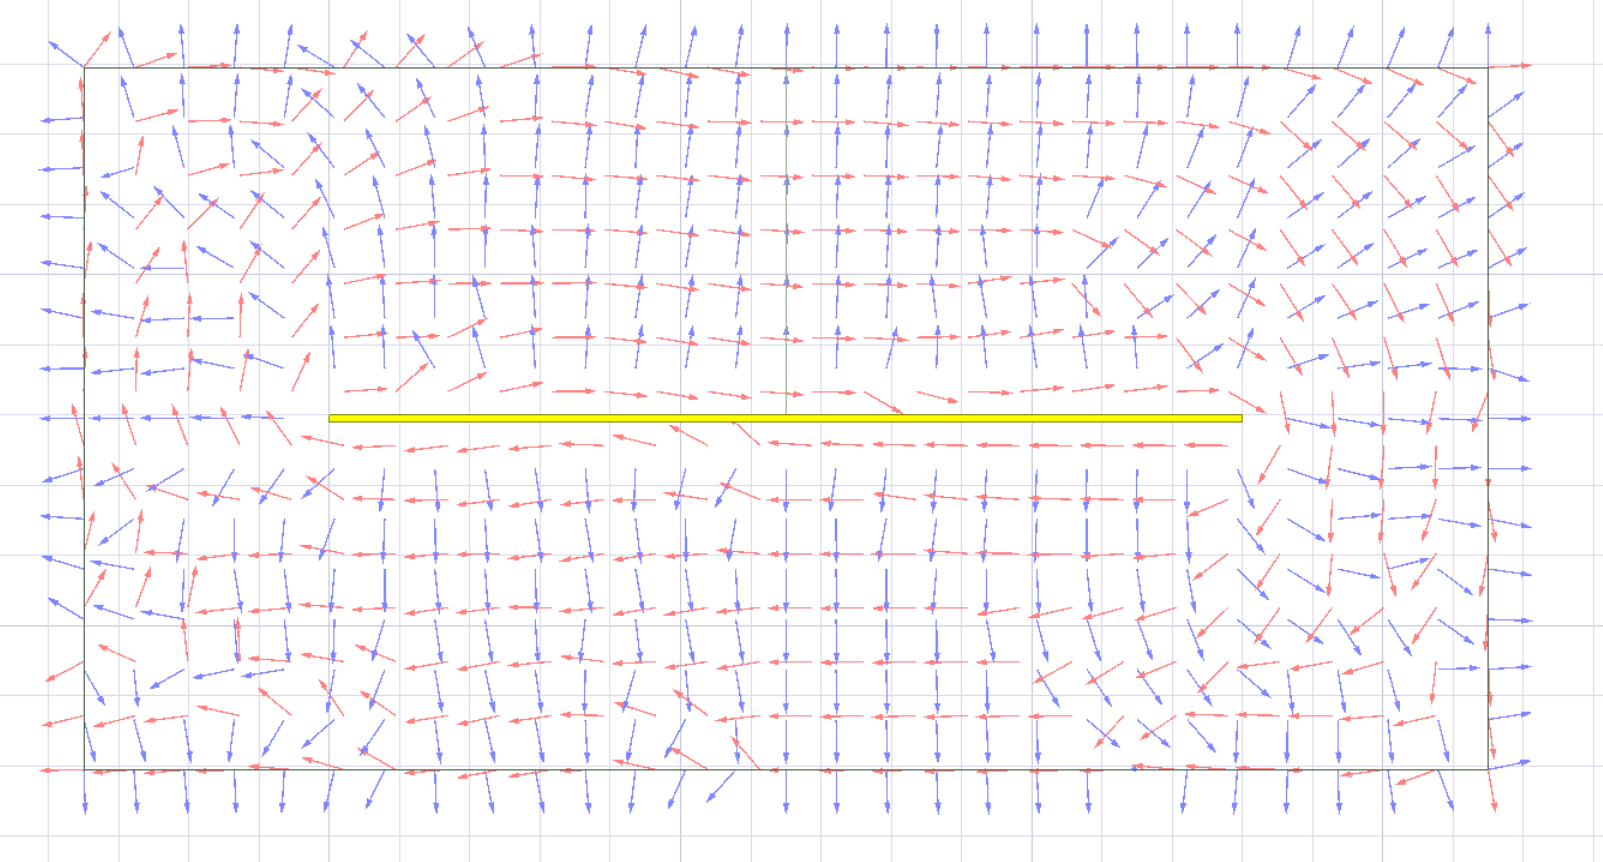
\includegraphics[width=0.5\linewidth]{images/tem_mode.png}
    \caption{TEM Mode}
    \label{fig:tem_mode}
\end{figure}
%(My TEM cell is too short to have more modes than this) Investigation of more modes would be interesting

The first mode after the TEM mode is the TE\textsubscript{01}


\subsection{Electrically Small Radiating Sources in TEM Cells}

% What is this subsection for? Maybe it should be combined with the TEM cell section. In there, the calculations with Green's theorem and Lorentz Reciprocity Theorem could be put. Then, the calculations from the paper of Sreenivasia could follow. It shows how to find the equivalent Dipole moments. It is important to know which modes are propagating. A Electric dipole, which points in direction of wave propagation, should not influence the result. However, it could create TM modes, which would transfer power to the ports. -> Investigate modes.

An electrically small radiating source may be represented by six dipoles. This number includes three magnetic dipoles pointing in every direction of the Cartesian coordinate system (x, y, and z-direction), and three electric dipoles in the same orientation. Consequently, an equipment under test (EUT) could be modeled with these dipoles, leading to much less computational effort in simulation. An analytical procedure to determine these dipole moments is presented by Sreenivasiah \cite{Sreenivasiah_Chang_Ma_1981}, and some experimental results based on it can be found in the research of Kreindl \cite{Kreindl_Bauernfeind_Weiss_Stockreiter_Kaltenbacher_2024} and, again, Sreenivasiah \cite{Sreenivasiah_Chang_Ma_1981}.

% Citing: "If the waveguide walls are perfectly conducting, the coefficients of such an expansion may be obtained in a straightforward manner, by an application of Lorentz's reciprocity principle." - This should be treated in the section about TEM cells. A reference to the Lorentz Reciprocity Theorem shall be made, and how it is used to determine the coefficients of the orthonormal modes.

The idea is to place the EUT in the TEM cell and measure the power of both output ports. The amplitudes of the TEM fields are expressed by \autoref{eqn:a_b_moments} \cite{Sreenivasiah_Chang_Ma_1981}. % maybe cut out this equation.

\begin{equation}
    \begin{pmatrix}a \\b\end{pmatrix} = \frac{1}{2}(-\mathbf{m_e}\cdot \mathbf{E_0}^\pm+\mathrm{i}\omega\mu_0\mathbf{m_m}\cdot\mathbf{H_0}^\pm)
    \label{eqn:a_b_moments}
\end{equation}

The magnetic field $\mathbf{H_0}$ and electric field $\mathbf{E_0}$ are both normalized to $1\,\sqrt{\mathrm{Hz}}$ \cite{Kreindl_Bauernfeind_Weiss_Stockreiter_Kaltenbacher_2024} and correspond to the TEM mode in free space \cite{Sreenivasiah_Chang_Ma_1981}. The electric dipole moment $\mathbf{m_e}$ and the magnetic dipole moment $\mathbf{m_m}$ are complex vectors, containing an amplitude and phase for every one of the three directions in the coordinate system (x, y, z), and have the units $\mathrm{A\cdot m}$ and $\mathrm{V\cdot m}$. This leads to the final form as \autoref{eqn:a_b_moments_simp} \cite{Sreenivasiah_Chang_Ma_1981}.

\begin{equation}
    \begin{pmatrix}a \\b\end{pmatrix} =-\frac{1}{2}(\mathbf{m_e\pm \mathrm{i}k\mathbf{m_m}\times \mathbf{z})\cdot \mathbf{e_0}}
    \label{eqn:a_b_moments_simp}
\end{equation}

The unity vector $\mathbf{z}$ points in direction of propagation. The function vector $\mathbf{e_0}$ describes the normalized electric field amplitude in traverse direction, i.e. x and y-directions, only, as it should have neither a z-component nor dependence. Due to the normalization of the electric and magnetic fields to $1\,\sqrt{\mathrm{Hz}}$, the total power at one port is 1\,W. This defines $\mathbf{e_0}$ as the electric field when the TEM cell is excited with unit power. 

Note, that an electric dipole in the TEM cell leads to a increase in power with the same phase in both ports, and a magnetic dipole leads to the same increase, but with a phase shift of 180°. This also explains why the EUT shall be place halfway on the septum in z-direction. Any shift from this position changes this phase shift from 180°. It is therefore required to measure the power of the ports with phase information, like using a complex Poynting vector, which is easy to implement in a simulation software. Additionally, only the electric or magnetic dipole, that is aligned with the electric or magnetic field in the TEM cell, influences the output power, ideally. In reality, at frequency which is high enough, the dipoles not aligned with the TEM mode will generate some TE/TM modes, which enable them to transmit power and disturb the results. Furthermore, in the optimal case, the EUT is placed in the dead center of the TEM cell, where the y-component of $\mathbf{e_0}$ in the x=0 plane becomes zero due to symmetry \cite{Sreenivasiah_Chang_Ma_1981}.

% The paper goes on to talk about the total power radiated by the EUT in free space. I don't think I need that, but this comment is here as a reminder that it exists.


\subsection{Shielding}

Effective shielding is of great interest to reduce EMI of electronic systems. A figure of merit for shielding capabilities of a material is the electromagnetic shielding effectiveness (SE), given in \autoref{eqn:se_elec_fields} \cite{10518640}. $E_\mathrm{i}$ is the incident electric field, while $E_\mathrm{t}$ is the transmitted electric field, also depicted in \autoref{fig:shielding_material_diagram}. It depends on the thickness and shape of the material, and its electric and magnetic properties. Addtionally, the TEM cell contributes to the SE values.

\begin{equation}
    SE_{\mathrm{dB}}=20\log{(\frac{E_\mathrm{i}}{E_\mathrm{t}})}
    \label{eqn:se_elec_fields}
\end{equation}

\begin{figure}[h]
    \centering
    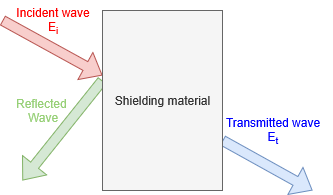
\includegraphics[width=0.35\linewidth]{Documentation//images/shielding_material_diagram.png}
    \caption{Incident, reflected and transmitted electric fields due to interaction with shielding material}
    \label{fig:shielding_material_diagram}
\end{figure}

Note: Higher order modes may not be able to propagate in the TEM cell, as the refraction of the shielding material follows to excitation of these modes.

% Quick mathematical formulation of how to calculate reflected waves?


\section{Antennas}
\subsection{Antennas to Investigate}

% List possible electrically short antennas to investigate with dipole moments here. Describe, why they are interesting.
% See: Crossed Dipole Antennas document by Bauernfeind

\subsubsection{IFA}
\subsubsection{Center fed monopole antenna}

\section{Simulations}
\subsection{Inverted F-antenna}\label{sec:ifa_sim}

The inverted F-antenna (IFA) is modeled in Ansys HFSS as shown in \autoref{fig:ifa}. Its material is copper. It is positioned at the center of the TEM cell, mounted at the top surface. The excitation is a modal wave port. With a maximum dimension of 2.7\,mm, the antenna is electrically small for a frequency of up to 11.1\,GHz, at which it will be a tenth of the wavelength. In this simulation, the antenna is investigated for a frequency of 550\,MHz, therefore, its size is by far small enough.

\begin{figure}[h]
    \centering
    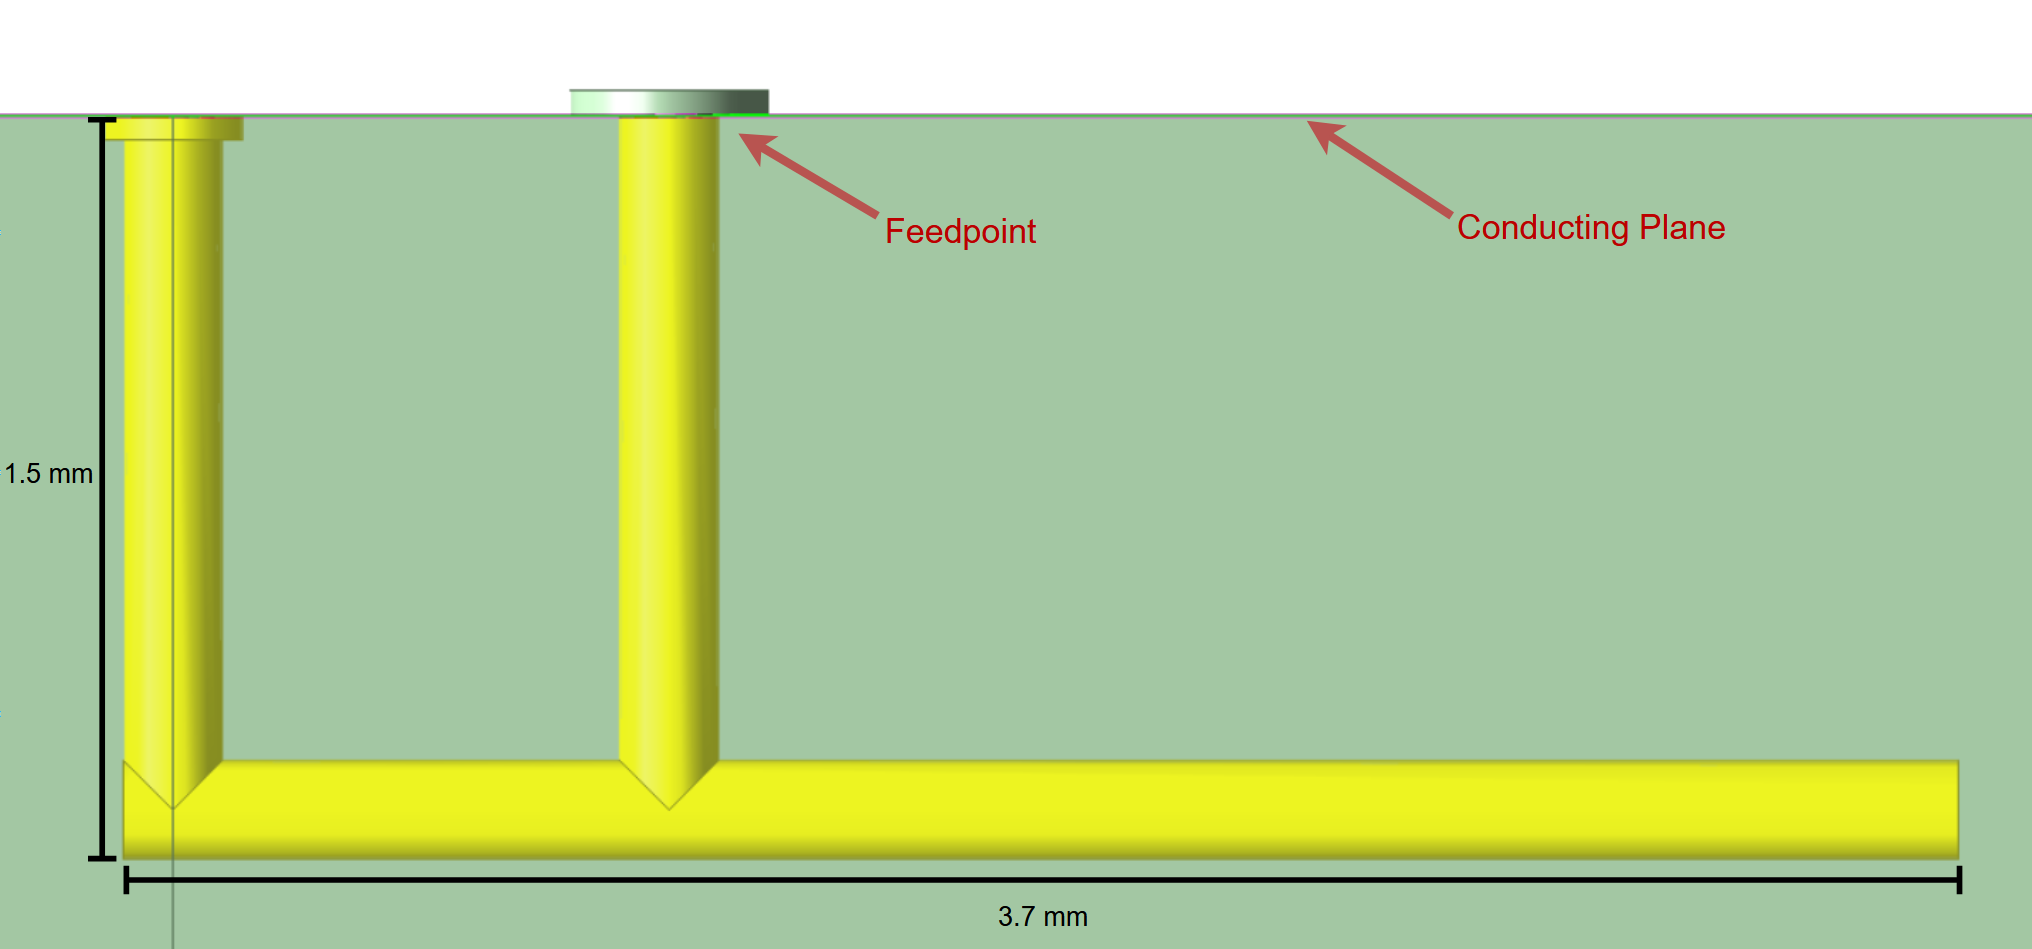
\includegraphics[width=0.7\linewidth]{Documentation//content//30_simulations//img/ifa.png}
    \caption{inverted F-antenna}
    \label{fig:ifa}
\end{figure}

The coupling between the antenna and the ports of the TEM cell are described by S-parameters. \autoref{fig:antenna_waveport1_sparams} and \autoref{fig:antenna_waveport1_sparams} show them for each ports, including the magnitude and phase. Specifically, the S-parameters at a frequency of 550\,MHz are marked, for which they are $S_{1\mathrm{A}}=3.337\cdot10^{-4}\cdot \mathrm{e}^{-\mathrm{i}\cdot151.85°}$ and $S_{2\mathrm{A}}=3.339\cdot10^{-4}\cdot \mathrm{e}^{\mathrm{i}\cdot40.76°}$. Note that the magnitude of the coupling is equal for each port, which is an inherent property of the electrically small antenna. Only the phase is different, which is due to the equivalent magnetic dipole.
 

\begin{figure}[h]
    \centering
    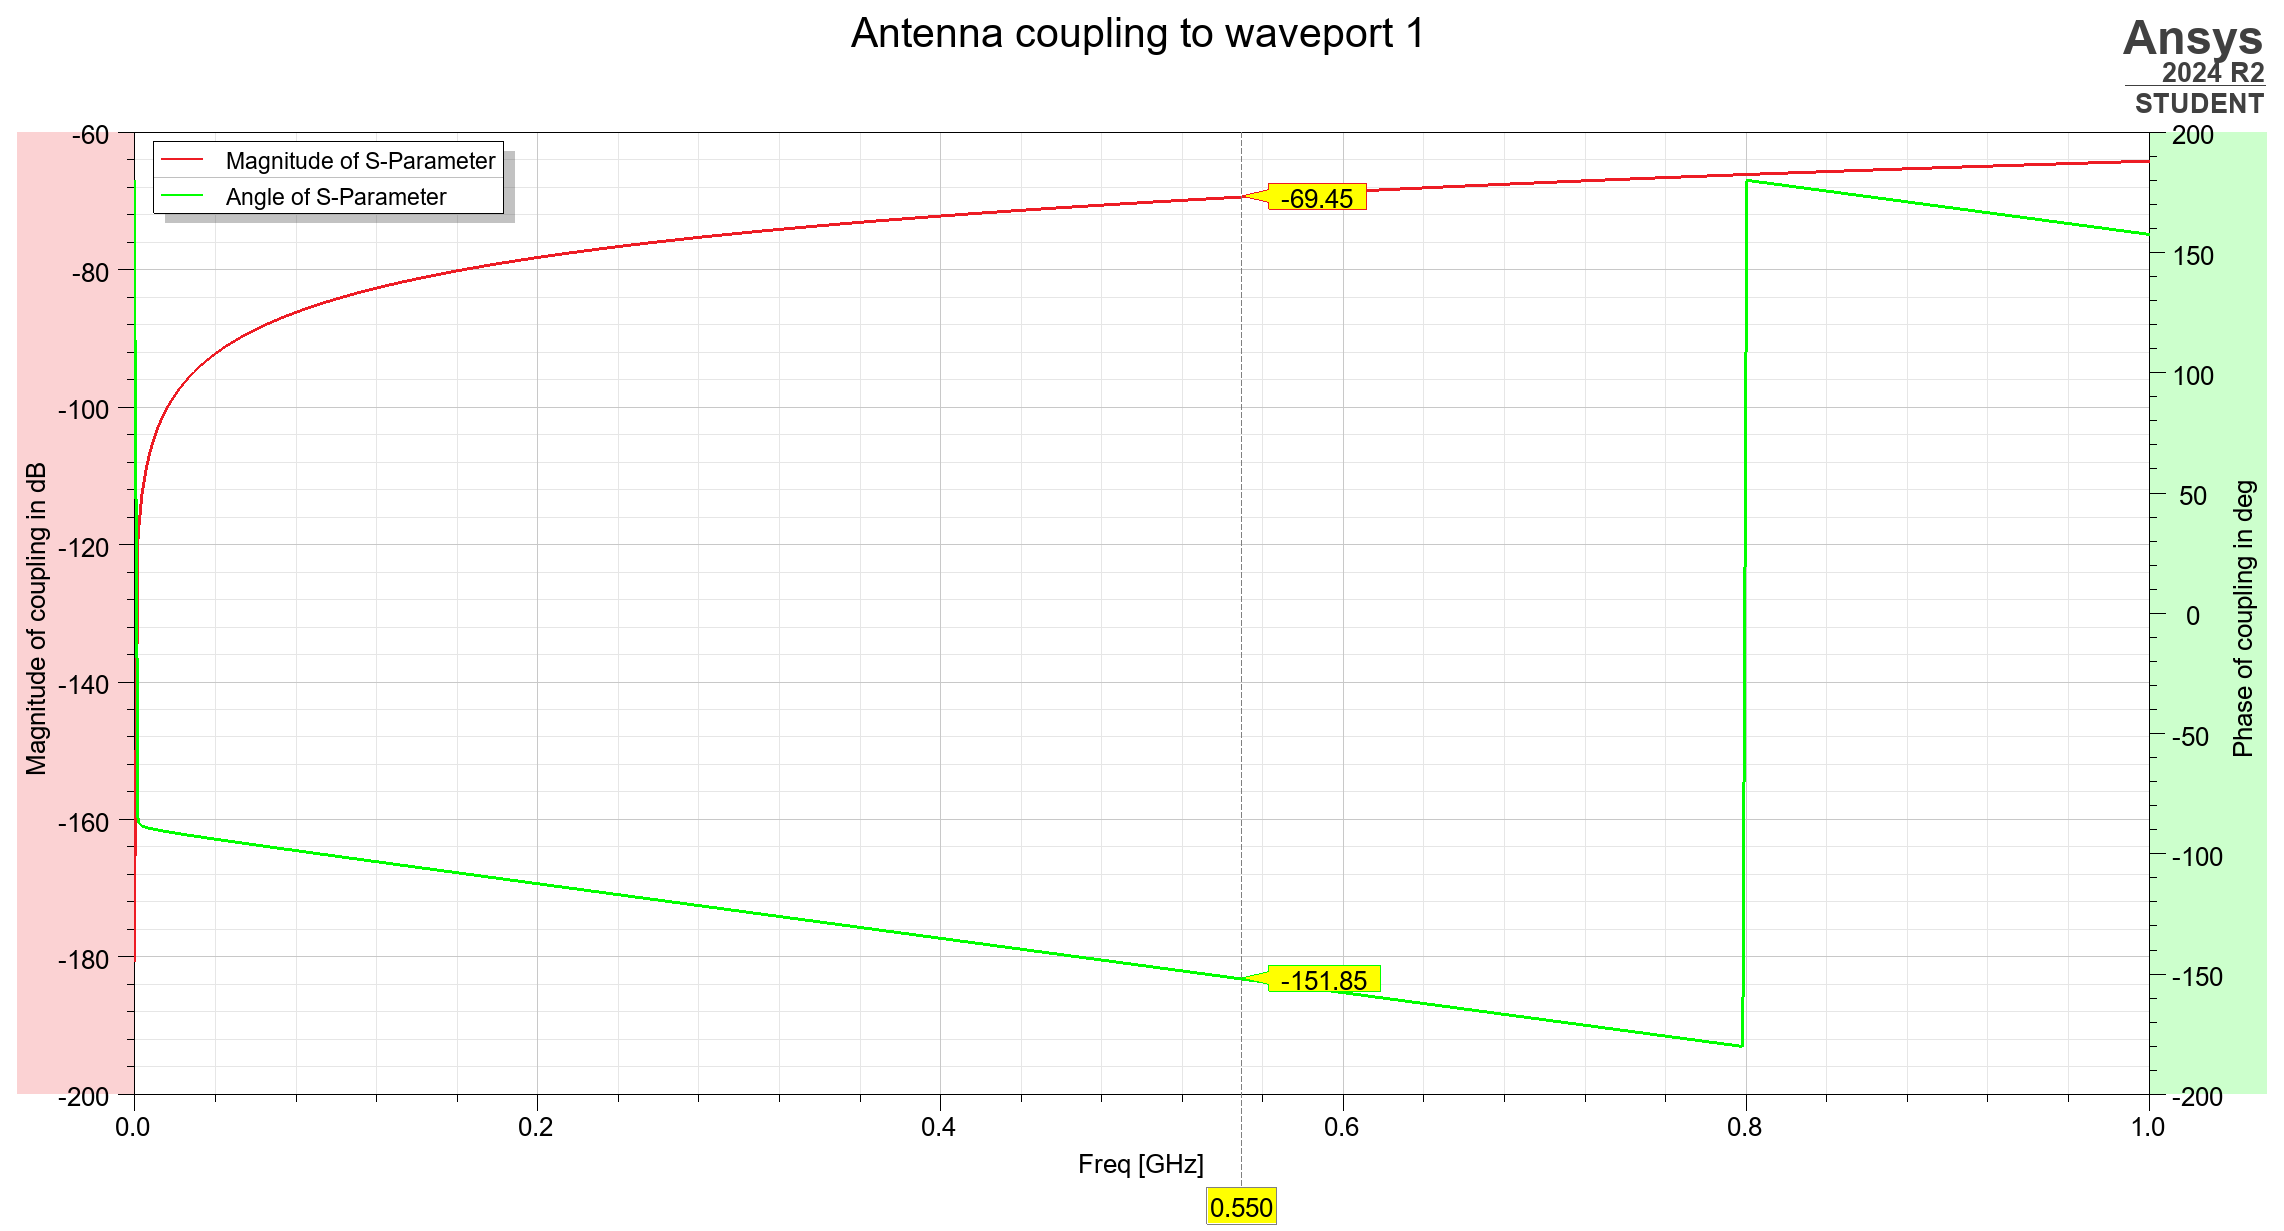
\includegraphics[width=1\linewidth]{Documentation//content//30_simulations//img/antenna_waveport1_sparams.png}
    \caption{S-Parameters describing coupling of antenna to waveport 1}
    \label{fig:antenna_waveport1_sparams}
\end{figure}

\begin{figure}[h]
    \centering
    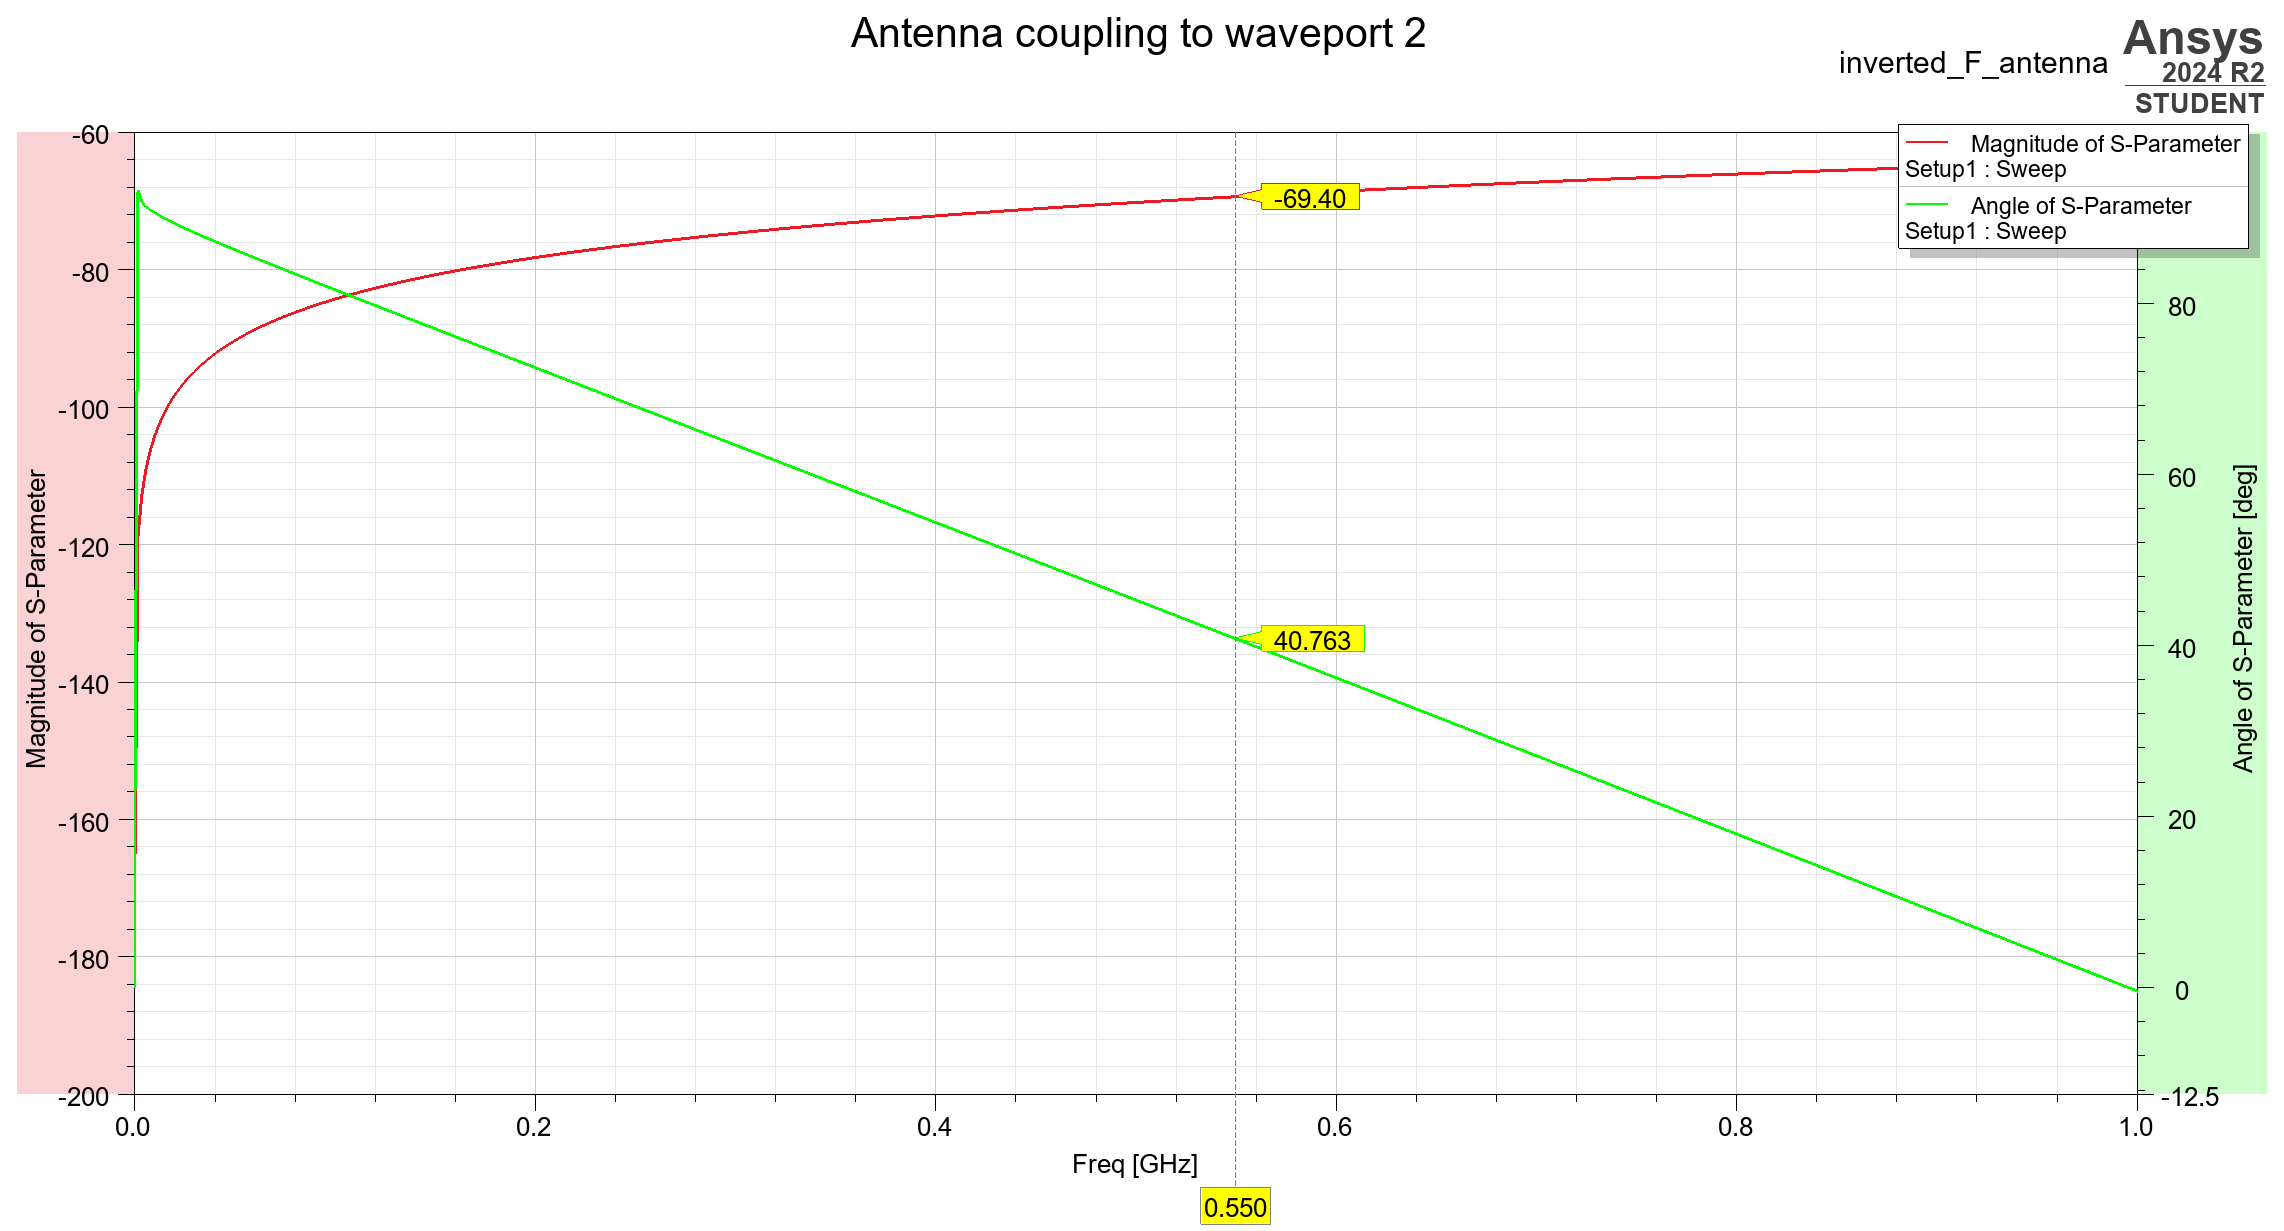
\includegraphics[width=1\linewidth]{Documentation//content//30_simulations//img/antenna_waveport2_sparams.png}
    \caption{S-Parameters describing coupling of antenna to waveport 2}
    \label{fig:antenna_waveport2_sparams}
\end{figure}

The measured electric field strength in z-direction at the center of the wave port is $E_{0,\mathrm{z}}=(-189.652 -\mathrm{i}\cdot66.529)\mathrm{\frac{V}{m}}$. It is much weaker in x- and y-direction, for which they will be ignored. The power at each output port is roughly 1\,W. Considering the the waves are sinusoidal, the amplitudes of the waves are $|a|=|b|=\sqrt{P}=2\,\mathrm{\sqrt{W}}$ with a phase-shift of 167.39° between them, which will be needed to calculate the dipole moments according to \autoref{eqn:a_b_moments_simp}. The crest-factor of $\sqrt{2}$ is used in the calculation of the wave amplitudes $a$ and $b$, which is squared due to the calculation with powers. The resulting dipole moments are displayed in \autoref{eqn:m_ez_ifa} and \autoref{eqn:m_my_ifa}.

\begin{align}
m_{\mathrm{ez}}&=2.198\cdot10^{-3}\cdot\mathrm{e}^{-\mathrm{i}\cdot124.99°}\mathrm{A\cdot m}\label{eqn:m_ez_ifa}\\
m_{\mathrm{my}}&=1.726\cdot10^{-3}\cdot\mathrm{e}^{-\mathrm{i}\cdot 124.99°}\mathrm{A\cdot m^2}\label{eqn:m_my_ifa}
\end{align}

Using \autoref{eqn:magn_current_curr_loop} the magnetic dipole moment can be expressed with a magnetic current. The resulting $m_{my,mag}$ is shown in \autoref{eqn:m_mymag_ifa}. Note that the phase shift between the magnetic and electric dipole moments $m_{\mathrm{ez}}$ and $m_{\mathrm{my,mag}}$ is exactly 90°, which creates a constructive interference pattern.

\begin{equation}
    m_{\mathrm{my,mag}}=\mathrm{i}m_{\mathrm{my}}\omega\mu_0=7.492\cdot\mathrm{e}^{-\mathrm{i}\cdot34.99°}\mathrm{V\cdot m}
    \label{eqn:m_mymag_ifa}
\end{equation}

Next, the antenna is replaced with those two dipole excitations in the center of the upper half of the TEM cell. The magnitude and phase of the fields is measured. The power going through each port is $1\,\mathrm{W}$, as expected. The phase shift is determined by measuring the phase of the electric fields at the center of both output ports and comparing them. It is 165.32°, which is very close to the value measured with the real antenna.

\subsection{Center Fed Monopole Antenna}

The same simulation procedure is repeated with a center fed monopole antenna. The parameters are listed in \autoref{tab:center_fed_monopole_params} for the chosen frequency of 550\,MHz. Interestingly, the electric dipole moment increased proportionally to the antenna's height in z-direction compared to the IFA in \autoref{sec:ifa_sim}, while the magnetic dipole moment remained roughly equal due to the unchanged loop area.
\todo{Next: Investigate how to set these dipoles over the frequency. They should be representable, independent of modes, when only looking at TEM mode. How does this change when several modes are able to propagate? Do I need to consider all 6 dipole moments, in order to represent such an antenna with dipole moments?}


\begin{table}[h]
    \centering
    \begin{tabular}{|c|c|}
        \hline
        Variable Name & Value\\\hline\hline
        $S_{1\mathrm{A}}$ & $3.51\cdot10^{-4}\cdot \mathrm{e}^{\mathrm{i}\cdot 48.86°}$\\\hline
         $S_{2\mathrm{A}}$&$3.49\cdot10^{-4}\cdot\mathrm{e}^{-\mathrm{i}\cdot 159.80°}$ \\\hline
         $E_{0,\mathrm{z}}$&$-189.652 -\mathrm{i}\cdot66.529\mathrm{\frac{V}{m}}$ \\\hline
         $m_{\mathrm{ez}}$&$4.926\cdot10^{-3}\cdot\mathrm{e}^{-\mathrm{i}\cdot74.8°}\cdot\mathrm{A\cdot m}$ \\\hline
         $m_{\mathrm{my}}$&$1.672\cdot10^{-3}\cdot\mathrm{e}^{-\mathrm{i}\cdot 74.8°}\cdot\mathrm{A\cdot m^2}$ \\\hline
         $m_{\mathrm{my,mag}}$&$7.264\cdot\mathrm{e}^{\mathrm{i}\cdot15.1994}\cdot\mathrm{V\cdot m}$ \\\hline
    \end{tabular}
    \caption{Determined parameters of the center fed monopole antenna}
    \label{tab:center_fed_monopole_params}
\end{table}





\newpage

\iffalse
\subsection{Summary}

\fi
\cleardoublepage
\printbibliography

\end{document}
